\documentclass[a4paper,12pt,twocolumn]{article}
\date{ }
\title{\textbf{Predicción del precio diario de Cierre del Bitcoin mediante Bagging, Árboles de decisión y Redes Neuronales. }}
\author{Vanessa Alcalde, Pablo Martinez Angerosa}
\usepackage[spanish]{babel}
\usepackage{graphicx}
\renewcommand{\figurename}{Figura}
\newtheorem{dfn}{Definición}
\renewcommand{\labelenumi}{P.\theenumi}
\renewcommand{\abstractname}{Resumen}
\renewcommand{\refname}{Bibliografía}
\renewcommand{\tablename}{Tabla} 
\usepackage{booktabs,xcolor,siunitx,amsmath }
\definecolor{lightgray}{gray}{0.9}

\begin{document}


\setlength{\columnsep}{0.8cm}
% now make the abstract span both columns
\twocolumn[
\maketitle

\begin{abstract}{
En 2008 Satoshi Nakamoto presentó una tecnología revolucionaria llamada Bitcoin. En evolución constante, el Bitcoin ya forma parte del interés diario de inversores y el mundo de la tecnología. Aquí presentamos una investigación que mediante  la comparación de distintas técnicas de Aprendizaje Automático (Bagging, Árboles de decisión y Redes Neuronales) establece a los algoritmos de Bagging empleados sobre Árboles de decisión como la opción con mejor desempeño entre estas técnicas para la predicción del precio de $Cierre$ de Bitcoin. 
\vspace{1.0cm}} 
\end{abstract}
]

\vspace{1.0cm}


\section{Introducción}
 Satoshi Nakamoto en 2008 presentó una tecnología revolucionaria~\cite{Satoshi}, que cambiaría la historia de la humanidad por siempre, mediante la publicación de un artículo que describía un sistema P2P (peer-to-peer) de dinero digital, llamado Bitcoin. 

El Bitcoin no es un simple cambio de modalidad, es un cambio de paradigma, que ha cobrado un impulso tal que, ha dejado de ser un tema de entusiastas en la criptografía a ser una realidad diaria, una opción de inversión real y parte de las noticias. Asimismo es el impulsor de una nueva tecnología llamada la cadena de bloques~\cite{Blockchain} (Blockchain) que es el fundamento tecnológico de las criptomonedas,  y que actualmente está revolucionando y ampliando las posibilidades del mundo tecnológico más allá de las criptos y el ecosistema tecnológico financiero~\cite{Bitcoin_revolucion_monetaria}. 

Esta moneda digital, fue creada en su propia arquitectura como una red descentralizada, un libro abierto de balance contable, donde todas las transacciones son públicas y verificadas mediante un proceso criptográfico realizado por los nodos de la misma red (miners), sin la necesidad de una casa centralizadora o un tercer interesado como agente de control y validación~\cite{Satoshi}. 

El objetivo de esta investigación es encontrar un modelo de predicción del precio diario de $Cierre$ del Bitcoin mediante la utilización de modelos de Aprendizaje Automático. 

Para esto se utilizaron modelos de regresión dado que la variable de interés es continua. Se emplearon técnicas de Árboles de decisión, Bagging y Redes Neuronales. 

Existen actualmente diversos artículos científicos para la predicción del precio del Bitcoin, pero comparado con predicciones tradicionales del Mercado de Valores esta sigue siendo un área inexplorada con mucho potencial y margen de investigación. La lectura de estos fue fundamental para la elección de variables y la selección de las técnicas aplicadas~\cite{mainDriversBitcoin}.

En la segunda sección de esta investigación detallamos la obtención y tratamiento de los datos, en la tercera sección describimos los modelos utilizados, en la cuarta sección presentamos los resultados y finalmente en la quinta sección mostramos las conclusiones de esta investigación y posibles trabajos a futuro.



\section{Datos}
\subsection{Descripción de los datos}

Para la construcción de la base de datos utilizamos los datos diarios del precio de $Apertura$, $Cierre$, $Volumen$ de transacciones, provistos por Cryptodatadownload\footnote{https://www.cryptodatadownload.com}  que mantiene actualizada las bases de precios diarios de las principales criptomenadas y las principales casas de cambio online. Para esta investigación se utilizaron los datos de la casa de cambio online Coinbase\footnote{https://www.coinbase.com} que es considerada una de las más seguras y estables por la comunidad, la cual permite la comercialización y respaldo de criptomonedas como Bitcoin, Ethereum y cuya sede se encuentra basada en USA. 

Se utilizaron los registros diarios en dólares americanos (USD)  de las criptomonedas Bitcoin(BTC), Ethereum(ETH), Litecoin(LTC), Bitcoin Cash(BCH), Ethereum Classic(ETC), Chainlink(LINK) y  Augur (REP). 

También se utilizaron los datos diarios provistos en Google Trends\footnote{https://trends.google.com/trends} que reflejan el grado de interés diario de la búsqueda de la palabra clave Bitcoin en el buscador de Google, siendo este el principal motor de búsqueda en la actualidad. El índice que provee estos datos mide el interés relativo de una búsqueda en una región dada y un intervalo de tiempo determinado. Según las explicaciones de Google un valor de 100 significa un pico en la popularidad del término buscado, un valor de 50 significa que el término es medianamente popular. Un resultado de 0 significa que no hay búsquedas suficientes en ese término. 

\subsection{Preparación de los datos}

La base de datos contiene 232 días comenzando en el día $22/1/2020$  hasta el $9/9/2020$. En la Figura~\ref{priceClose} se muestran los datos del $Cierre$ del Bitcoin como serie temporal en este intervalo de tiempo. 

\begin{figure*}[!hbt]
\centering
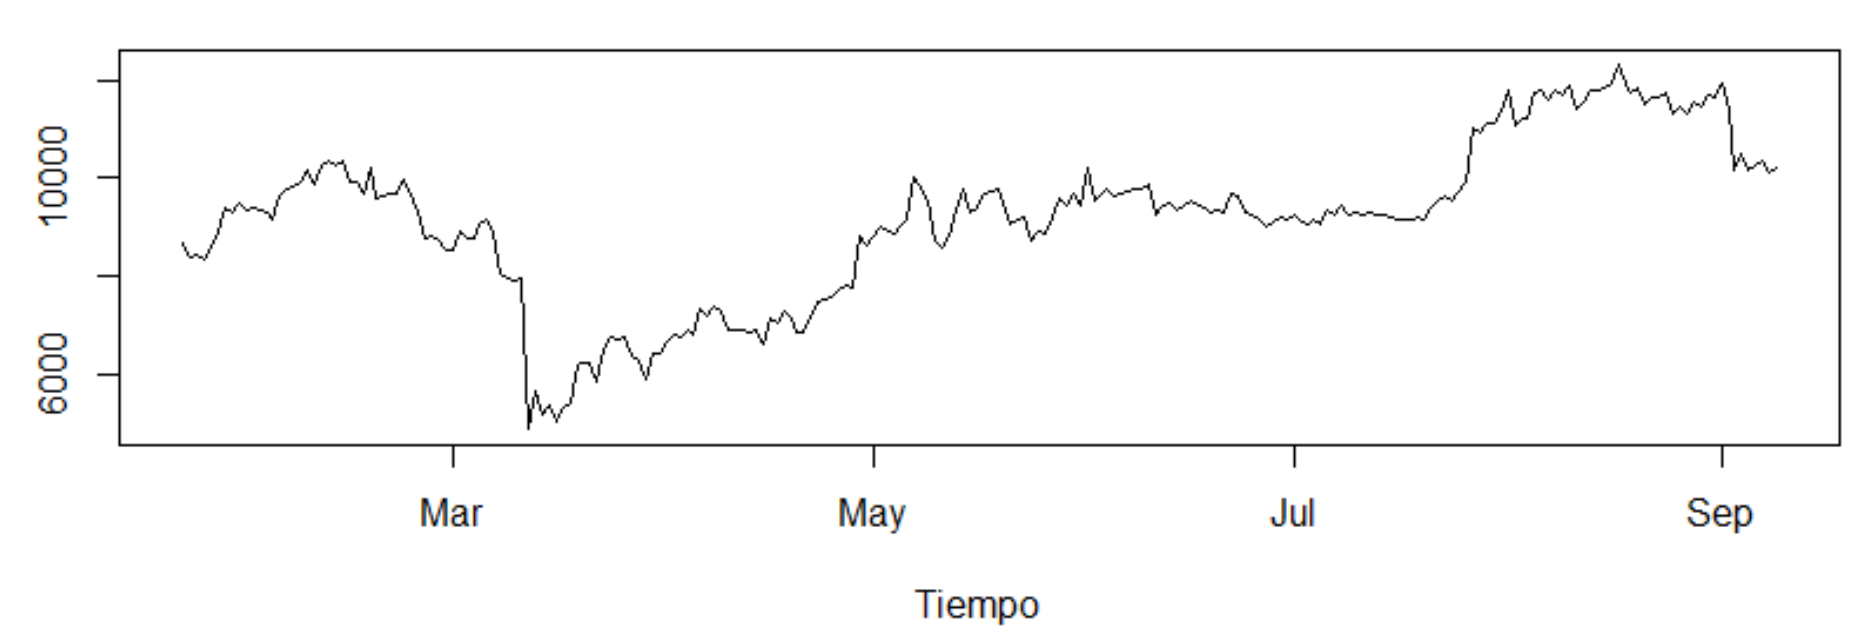
\includegraphics[width=1\textwidth]{priceCloseBitcoin}
\caption{Serie de tiempo del precio del Cierre del Bitcoin desde el día $22/1/2020$  hasta el $9/9/2020$.}
\label{priceClose}
\end{figure*}

Todas las bases provistas por Cryptodatadownload se encuentran en formato de archivo .CSV y no requirieron mayor preparación ya que no existían datos faltantes y el formato es ampliamente utilizado. 

Para armar la variable de Google Trends fue necesaria la implementación recursiva de la descarga de la base de datos en distintas ventanas de tiempo para una unión posterior de los datos. Esto es debido a que la información diaria provista por Google tiene un marco de ventana de dos meses. 

La base se estructuró de modo de tener un conjunto de entradas $X$ y salidas $Y$ con una dependencia temporal. La variable de predicción $Y$ corresponde al $Cierre$ del precio del Bitcoin en el tiempo $n$. Las entradas correspondientes a $X$ se encuentran en diversos momentos del pasado. 

Todos los precios de $Apertura$ se encuentran en el mismo tiempo $n$ que se quiere predecir, ya que para realizar la predicción es información que existe en ese momento. 

Todas las variables $Volumen$ correspondientes a las distintas monedas corresponden al tiempo $n-1$ ya que es información que no existe a la hora de predecir el momento $n$.

También se crearon variables  de retraso llamadas $lag$, para el precio de $Cierre$ y $Volumen$ de Bitcoin. Los números utilizados para nombrar las variables de retraso, representan el tiempo del pasado. Por ejemplo la variable $closeLag3$ representa el precio del $Cierre$ del Bitcoin 3 días previos al momento $n$~\cite{forecastinBitcoinClosing}.  

\section{Los modelos}

Las tres técnicas utilizadas en esta investigación incluyen Árboles de decisión, Bagging y Redes Neuronales. Todas se utilizan exclusivamente desde una perspectiva de predicción del precio de $Cierre$ del Bitcoin. 

Un árbol de decisión es una división recursiva del espacio de variables explicativas en una estructura en forma de árbol, cada nodo interior contiene una pregunta sobre una variable de entrada y cada nodo terminal una decisión. Estos pueden ser utilizados en problemas de regresión y clasificación, en nuestro caso la variable explicada es continua por lo que trabajamos con un árbol de regresión.  

Los árboles CART (Classification And Regression Tree) se construyen dividiendo el conjunto de valores posibles de $X_1,X_2,...,X_p$ en $J$ regiones disjuntas $R_1, R_2,..., R_J$. En el caso de un árbol de regresión, para cada observación en la región $R_j$ se predice el valor medio de las respuestas.

Para llevar a cabo la construcción del árbol se comienza con un conjunto de datos de entrenamiento, el cual es segmentado mediante particiones binarias. Se crean regiones $R_1, R_2,..., R_J$ de manera que se minimice la siguiente ecuación.

$$
\sum_{j=1}^{J} \sum_{i \in R_{j}}\left(y_{i}-\hat{y}_{R_{j}}\right)^{2}
$$

Donde $\hat{y}_{R_{j}}$ es la respuesta media para las observaciones del conjunto de entrenamiento en la región j-ésima~\cite{libroCurso}.

Una vez que se encuentra la mejor partición, se separan los datos en las regiones resultantes y se repite el proceso. Este proceso termina cuando se satisface algún criterio de parada.

El método Bagging (Bootstrap Aggregating) es un procedimiento para reducir la varianza de un modelo de aprendizaje automático~\cite{libroCurso}.

Se divide el conjunto de datos en entrenamiento $L$ y testeo $T$, se toma una muestra bootstrap $L_b$ de $L$ y se construye un estimador usando $L_b$. Se repite el procedimiento $B$ veces. Luego a cada dato de $T$ se le asigna el promedio de las respuestas de los estimadores construidos en el paso anterior (para el caso de un modelo de regresión). La proporción de veces que la clase estimada difiere de la verdadera es el error Bagging. Luego puede repetirse la división de los datos en $L$ y $T$ varias veces y calcular los errores promedio.

Bagging puede ser utilizado para Árboles de decisión, para esto se construyen $B$ árboles con conjunto de entrenamiento obtenido mediante una muestra bootstrap del conjunto de entrenamiento original, luego se hace un promedio de las predicciones resultantes. Estos árboles tienen varianza grande pero sesgo bajo ya que no se podan. Al promediarlos se reduce la varianza y por lo tanto se mejora la precisión de las predicciones.

Las Redes Neuronales son un modelado matemático que homologa el comportamiento de una neurona biológica. El objetivo de su diseño es emular al cerebro humano. Básicamente   se basa en una red  de neuronas conectadas que reciben un estímulo de entrada y producen una salida.   

En su modelado matemático se construyen combinaciones lineales de las entradas y se obtiene la salida como una función no lineal de estas. 

En la Ecuación (\ref{ecuacionRedes}) se muestra el modelado de una red neuronal con una capa de entrada, una capa oculta  y una salida. Donde $i$,$j$ son los índices correspondientes a la capa de entrada y oculta respectivamente, $w$ corresponde a los pesos de cada neurona y $f(.)$ a la función de activación.

\begin{equation}
g_{k}(x)=f \underbrace{(\sum_{j=1}^{n_{H}} w_{k j} f \underbrace{\left(\sum_{i=1}^{d} w_{j i} x_{i}+w_{j 0}\right)}_{\text {net }_{j}}+w_{k 0})}_{\text {net }_{k}}
\label{ecuacionRedes}
\end{equation}

En la Figura~\ref{redNeuronal} se muestra la arquitectura de una neurona simple. El procedimiento para encontrar los pesos que configuren el mejor modelo consiste en primero multiplicar cada dato de entrada por un peso y los valores ponderados se combinan linealmente. Posteriormente se aplica una función de activación no lineal. El valor de salida es comparado con el valor objetivo. La diferencia de error que se produce es utilizada para actualizar los pesos y se itera hasta obtener el criterio deseado de parada. Actualmente el algoritmo más utilizado para esto es el de Backpropagation.  Esta arquitectura crece en complejidad pero el algoritmo y los procesos son siempre los mismos. 

\begin{figure}[!hbt]
\centering
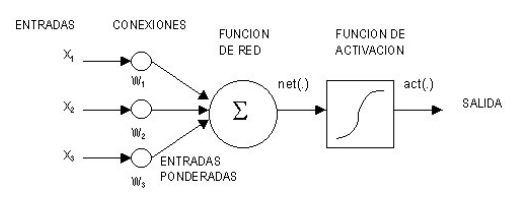
\includegraphics[width=0.5\textwidth]{redNeuronal}
\caption{Arquitectura donde se muestra una red neuronal simple, con una capa de entrada, una capa oculta y una capa de salida. Adoptado de Neurona, 2008 (https://poncos.wordpress.com/2008/03/
17/introduccion-a-las-redes-neuronales/).}
\label{redNeuronal}
\end{figure}

En el caso de Árboles de decisión y Bagging para encontrar el modelo con mejor  desempeño se construyó un algoritmo de fuerza bruta que evalúa secuencialmente una a una todas las posibles combinaciones de variables para generar un modelo de predicción. Este modelo se corrió en distintas combinaciones fijadas manualmente (por intento y error) de posibles grupos de variables, ya que el orden de todas las combinaciones es de $2^n - 1$ para $n$ opciones de variables. Y para $n>20$ el algoritmo se vuelve computacionalmente costoso.

\begin{equation}
(min)RMSE=\sqrt{\frac{1}{N} \sum_{i=1}^{N}\left(y_{i}-f_{i}\right)^{2}}
\label{remseequation}
\end{equation}

Para evaluar el desempeño de los distintos modelos de predicción se utilizó la medida de error RMSE como se ve en la Ecuación (\ref{remseequation}) donde $y_i$ representa las predicciones y $f_i$ los valores reales. Se busca minimizar el RMSE.


El conjunto de datos se dividió aleatoriamente, en una muestra de entrenamiento del $70\%$ y una muestra de testeo del $30\%$.


\section{Resultados}

El objetivo de  esta investigación es evaluar la predicción del precio de $Cierre$ del Bitcoin mediante algoritmos de Aprendizaje automático. 

En primer lugar, para el caso de Árboles de regresión y Bagging se buscó encontrar el modelo con menor RMSE mediante un algoritmo de fuerza bruta. Este algoritmo evalúa todos los posibles modelos generados a partir de todas las combinaciones posibles de 12 variables seleccionadas mediante prueba y error. Estas variables son $trend$ (las tendencias de búsqueda en Google), $ltcOpen$ (precio de $Apertura$ de Litecoin), $closeLag1$, $closeLag2$, $closeLag3$, $closeLag4$, $closeLag5$ (cinco primeros retrasos del precio de $Cierre$ de Bitcoin), $volLag1$, $volLag2$, $volLag3$, $volLag4$, $volLag5$ (cinco primeros retrasos del $Volumen$ de Bitcoin). Para estas técnicas se utilizó el paquete randomForest~\cite{randomForest} de R~\cite{r}.

En la Figura ~\ref{decisionTree}  se muestra el Árbol de regresión con menor RMSE obtenido para predecir el precio de Cierre del Bitcoin basado en el retraso del Cierre de un día. La división en la parte superior del árbol da como resultado dos ramas grandes. A modo de ejemplo, la rama de la izquierda corresponde a $closeLag1<8182$, lo que representa al $22\%$ de las observaciones, y la rama de la derecha corresponde a $closeLag1 \geq 8182$, el $78\%$ de las observaciones. La rama izquierda se vuelve a dividir. La nueva rama izquierda representa las observaciones que tienen un $closeLag1<6415$, el $7\%$ de ese $22\%$ inicial; y la rama derecha representa las observaciones que tienen un  $closeLag1 \geq 6415$ y además un $closeLag1<8182$, estas son el $15\%$ restante de las observaciones. Estos últimos dos nodos son llamados terminales u hojas y el número en cada una de estas es la media de la respuesta de las observaciones que se encuentran allí. Este árbol tiene cuatro nodos internos y cinco nodos terminales u hojas.

Es importante recalcar que de los $4095$ ($2^{12} - 1$) posibles modelos resultantes por el algoritmo de fuerza bruta, $2048$ modelos obtienen el menor RMSE de $537.6748$. En este caso por el principio de parsimonia se selecciona el modelo con menor cantidad de variables, el cual sólo consta de una variable que es el primer retraso del precio de $Cierre$ del Bitcoin. 
Esto es un punto interesante, ya que como se menciona en~\cite{forecastinBitcoinClosing}, esto confirma la hipótesis que la serie del precio del Bitcoin en su medida histórica global es indistinguible de un paseo aleatorio. 

\begin{figure}[!hbt]
\centering
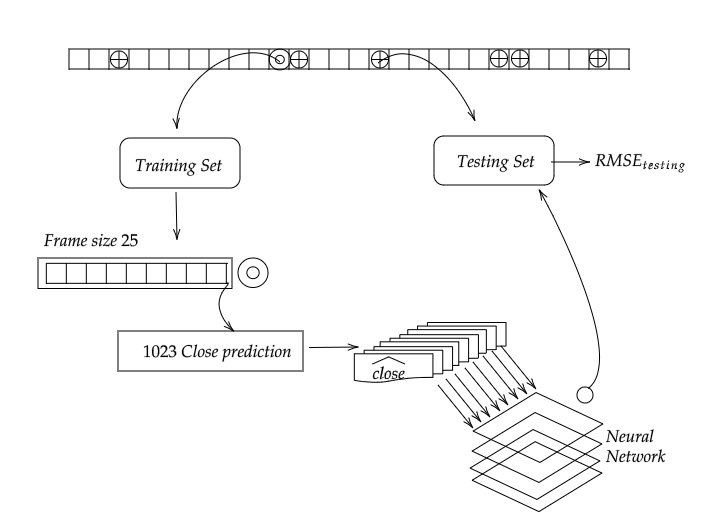
\includegraphics[width=0.5\textwidth]{diagramNeuralNetwork}
\caption{Árbol de regresión correspondiente al precio de Cierre del Bitcoin.}
\label{decisionTree}
\end{figure}

En el caso de Bagging el modelo que logra un menor RMSE de $454.5812$ está compuesto por las variables $trend$, $closeLag1$, $closeLag2$, $closeLag3$, $volLag3$, $volLag5$ y $ltcOpen$. En el Cuadro~\ref{baggingTop10} se muestran los diez modelos que lograron el menor RMSE con esta técnica. En la Figura~\ref{baggingVariableImportancia}  se muestra la media de precisión en las predicciones en la muestra cuando cada una de las variables se excluye del modelo. Es interesante como se destaca la importancia de la variable $closeLag1$ con respecto a las demás variables que forman el modelo, siendo esto concluyente con la hipótesis previamente mencionada de que el precio del Bitcoin es un camino aleatorio. 


\begin{figure*}[!hbt]
\centering
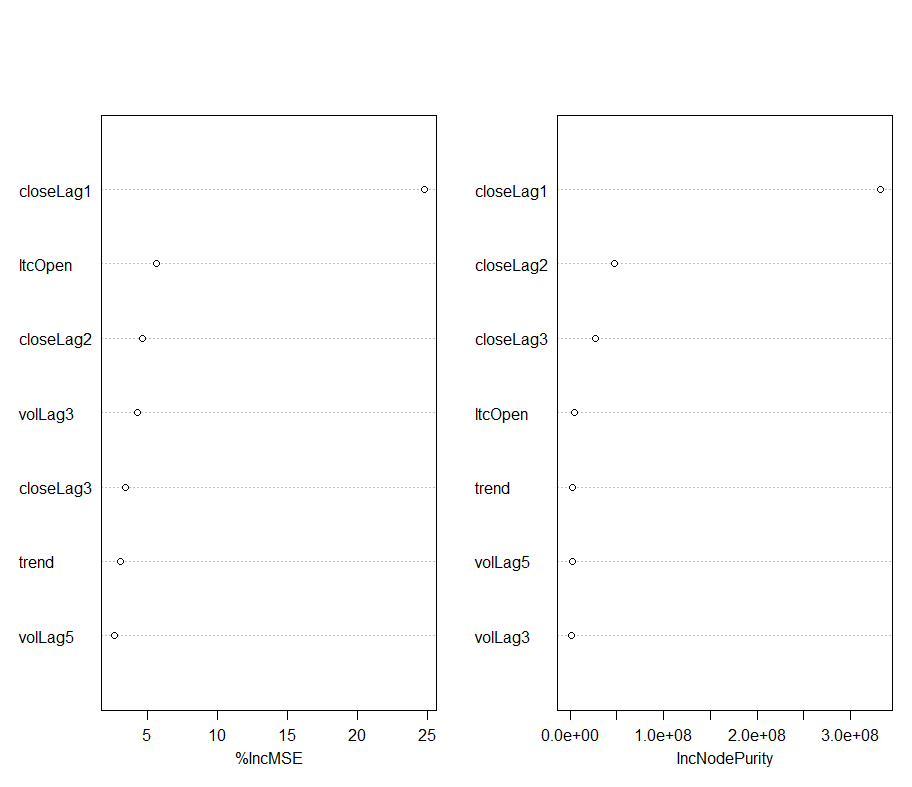
\includegraphics[width=0.7\textwidth]{baggingVariableImportancia}
\caption{A la izquierda se muestra la disminución media de la precisión en las predicciones en la muestra OOB cuando una variable determinada se excluye del modelo (IncMSE). A la derecha se muestra la disminución total en la impureza del nodo que resulta de las divisiones sobre esa variable, promediada en todos los árboles para regresión (IncNodePurity).}
\label{baggingVariableImportancia}
\end{figure*}

Otro indicador de error de prueba es el error out-of-bag (OOB). Los árboles que se construyen en Bagging se generan con muestras bootstrap que utilizan aproximadamente dos tercios de las observaciones originales, las restantes son llamadas out-of-bag. Para el caso de regresión se puede calcular el RMSE OOB, este sirve como una estimación del error de prueba debido a que la respuesta para cada observación se predice utilizando solamente los árboles que no se ajustaron con dicha observación. Este es incluso una aproximación al error de validación cruzada dejando uno fuera cuando el número de árboles es suficientemente grande, en nuestro caso el número de árboles empleados es de 100. Aplicando el RMSE OOB en el modelo final de Bagging se obtiene un resultado de $467.7928$. Esto nos da a entender que el modelo en otras circunstancias de predicción sigue teniendo un comportamiento similar ya que la diferencia con el RMSE es baja.

\begin{table*}[!hbt]
\centering
\caption{Variables utilizadas para los mejores 10 modelos y su RMSE correspondiente para la predicción del precio de $Cierre$ de Bitcoin utilizando Bagging.}
\label{baggingTop10}
\begingroup\setlength{\fboxsep}{0pt}
\colorbox{lightgray}{%
\begin{tabular}{|l|l|}
\hline Modelo & RMSE \\
\hline  trend, closeLag1, closeLag2, closeLag3, volLag3, volLag5, ltcOpen & 454.5812\\
\hline trend, closeLag1, closeLag3, volLag2, volLag3, volLag4, volLag5, ltcOpen & 456.4094 \\
\hline   trend, closeLag1, closeLag3, closeLag4, closeLag5, volLag1, volLag3, \\volLag4, volLag5, ltcOpen& 459.2152 \\
\hline  trend, closeLag1, closeLag2, closeLag4, volLag3, volLag4, volLag5& 459.6356 \\
\hline  trend, closeLag1, closeLag2, closeLag3, closeLag4, volLag3, volLag5& 459.7546\\
\hline trend, closeLag1, closeLag2, closeLag3, volLag2, volLag3, volLag5, \\ ltcOpen & 459.7760\\
\hline trend, closeLag1, closeLag3, volLag1, volLag3, volLag4, volLag5, \\ ltcOpen & 460.0010\\
\hline trend, closeLag1, closeLag2, closeLag4, volLag3, volLag5, ltcOpen & 460.0387\\
\hline trend, closeLag1, closeLag3, closeLag4, volLag1, volLag2, volLag3, \\ volLag4, volLag5, ltcOpen & 460.5488\\
\hline trend, closeLag1, closeLag3, closeLag5, volLag1, volLag2, volLag3, \\ volLag4, volLag5, ltcOpen & 460.6552\\
\hline
\end{tabular}%
}\endgroup
\end{table*}

Para las Redes Neuronales se utilizó el paquete Keras~\cite{keras} de R~\cite{r} que es una capa de alto nivel de Tensorflow~\cite{tensorflow}. Tensorflow es una biblioteca de código abierto propiedad de Google y de las más utilizadas actualmente para el aprendizaje profundo. En el Cuadro~\ref{redesModelTuning} se muestran los RSME obtenidos por distintas configuraciones de capas y funciones de activación. En particular para todas las redes se utilizaron las mismas variables de entrada  las cuales son las obtenidas por el modelo con menor RMSE de Bagging ($trend$, $closeLag1$ , $closeLag2$ , $closeLag3$ ,  $volLag3$ , $volLag5$ y $ltcOpen$). Todas las redes constaban de 3 capas ocultas, donde la primera capa oculta es utilizada para la estandarización de los valores de las variables de entrada. La segunda capa oculta se probó con 8 y 16 nodos y funciones de activación linear y relu. La  tercer capa se probó con 8 nodos y funciones relu. La tendencia de los nodos y capas probados mostraron que al agregar más nodos en las capas se obtenían mejores resultados. Estos algoritmos emplean una gran cantidad de procesos informáticos, por lo que probar con más nodos y capas, exigía un poder computacional fuera del alcance técnico empleado para esta investigación. 


\begin{table*}[!hbt]
\centering
\caption{Combinaciones de banderas utilizadas en las Redes Neuronales y el RMSE obtenido para la predicción del $Cierre$ de Bitcoin. }
\label{redesModelTuning}
\begingroup\setlength{\fboxsep}{0pt}
\colorbox{lightgray}{%
\begin{tabular}{|l|l|l|l|l|}
\hline Capa de nodos 2 & Capa de nodos 3 & Capa de activación 2 & Capa de activación 3 & RMSE \\
\hline 16& 8 & linear & relu  &  485.0457\\
\hline 16& 8 & relu & relu  &  546.5264\\
\hline 8& 8 & relu & relu  &  610.5063\\
\hline 8& 8 & linear & relu  & 2657.04\\
\hline
\end{tabular}%
}\endgroup
\end{table*}

En el Cuadro~\ref{RMSEFinal} se muestra el desempeño de cada uno de los modelos seleccionados por las técnicas empleadas (Bagging, Árboles de decisión y Redes Neuronales). En este caso el modelo seleccionado para Bagging es el que logra mejores resultados. A la vez la tabla muestra, como la flexibilización del algoritmo, no necesariamente arroja mejores resultados. También en nuestra investigación anterior~\cite{paper1}, donde se utilizaron algoritmos de Aprendizaje Automático menos flexibles, los RMSE obtenidos son ampliamente menores que los de esta investigación. En particular con Modelos Lineales se logra un RMSE de $291.971$.

En el caso de Modelos Lineales las variables que se obtuvieron en el modelo fueron $trend$, $closeLag1$, $closeLag2$, $closeLag4$,  $volLag1$, $volLag3$, $volLag4$ y $ltcOpen$. Es interesante notar que solo existen diferencias de los valores de retrasos pero las variables son las mismas que en el modelo obtenido por Bagging en esta investigación. 

\begin{table}[!hbt]
\centering
\caption{Mejores resultados de RMSE obtenidos para las tres técnicas utilizadas en la predicción del $Cierre$ de Bitcoin. }
\label{RMSEFinal}
\begingroup\setlength{\fboxsep}{0pt}
\colorbox{lightgray}{%
\begin{tabular}{|l|l|}
\hline Algoritmo de predicción & RMSE \\
\hline Bagging (Árbol de decisión)& 454.5812\\
\hline Redes Neuronales & 485.0457 \\
\hline Árbol de decisión & 537.6748 \\
\hline
\end{tabular}%
}\endgroup
\end{table}
   
\section{Conclusiones}

Los resultados obtenidos muestran que entre los métodos utilizados en esta investigación, la técnica de Bagging es la que obtiene mejores resultados para la predicción del precio de $Cierre$ del Bitcoin. Sin embargo, estos métodos más flexibles no obtuvieron mejores resultados que estudios previos con modelos menos flexibles, en particular Modelo Lineales. 

A futuro se plantea la posibilidad de utilizar Bagging para estabilizar los modelos obtenidos de Redes Neuronales. También se mostró una tendencia a la mejora del desempeño en cuanto se aumentaba la cantidad de nodos y conexiones en las Redes Neuronales, por lo que probar modelos con más capas, nodos y conexiones complejas, es una opción a investigar en próximas instancias.
     

\newpage  
\onecolumn              
%
\begin{thebibliography}{99}

\bibitem{Bitcoin_revolucion_monetaria}
Sangoi, F.
{\em Bitcoin. ¿Una revolución monetaria?}
Universidad de Buenos Aires.
%
\bibitem{regression_for_bitcoin_price}
Azim Muhammad Fahmi, Noor Azah Samsudin, Aida Mustapha, 
Nazim Razali, Shamsul Kamal Ahmad Khalid. (2018).
{\em Regression based Analysis for Bitcoin Price Prediction.}
Faculty of Computer Science and Information Technology, Universiti Tun Hussein Onn Malaysia.

\bibitem{Satoshi}
Nakamoto, S. (2008).
{\em Bitcoin: A Peer-to-Peer Electronic Cash System.}

\bibitem{Blockchain}
Carlos Dolader Retmal et al.
{\em La blockchain: fundamentos, aplicaciones y relación con otras tecnologías disruptivas}, Universitat Politécnica de Catalunya.

\bibitem{Blockchain_science}
Karame, G., Huth, M., Vishik, C. (2020).
{\em An overview of blockchain science and
engineering.} R. Soc. Open Sci. 7: 200168.
http://dx.doi.org/10.1098/rsos.200168


\bibitem{Bayesian}
Shah, D., Zhang, K. (2014).
{\em Bayesian regression and Bitcoin.} 
Laboratory for Information and Decision Systems
Department of EECS, Massachusetts Institute of Technology.


\bibitem{Methods}
Ferdiansyah, Siti Hajar Othmanb, Raja Zahilah Raja Md Radzic, Deris Stiawan. (2019).
{\em A Study of Bitcoin Stock Market Prediction: Methods, Techniques and Tools.} 

\bibitem{Bitcoin_bubbles_predictable}
Wheatley, S., Sornette, D., Huber, T., Reppen, M., Gantner, RN. (2019). 
{\em Are Bitcoin bubbles predictable? Combining a generalized
Metcalfe’s Law and the Log-Periodic Power Law
Singularity model.} R. Soc. open sci. 6: 180538.
http://dx.doi.org/10.1098/rsos.180538

\bibitem{forecastinBitcoinClosing}
Uras, N., Marchesi, L., Marchesi, M., Tonelli, R. (2020)
{\em Forecasting Bitcoin closing price series using linear
regression and neural networks models}. Department of Mathematics and Computer Science,
University of Cagliari.

\bibitem{forecast_bitcoin_GAM}
Asante Gyamerah, S. (2020).
{\em On forecasting the intraday Bitcoin price using ensemble of variational
mode decomposition and generalized additive model}. Pan African University, Institute for Basic Sciences, Technology, and Innovation.
https://doi.org/10.1016/
j.jksuci.2020.01.006


\bibitem{bitcoin_ML}
McNally, S. (2016).
{\em Predicting the price of Bitcoin using Machine Learning.} School of Computing National College of Ireland.

\bibitem{mainDriversBitcoin}
Kristoufek, L. (2015). {\em What Are the Main
Drivers of the Bitcoin Price? Evidence from Wavelet
Coherence Analysis.} PLoS ONE 10(4): e0123923.
doi:10.1371/journal.pone.0123923

\bibitem{bitcoin_ML_PSA}
Rajua, S., Mohammad, A. (2020).
{\em Real-Time Prediction of BITCOIN Price using Machine Learning Techniques and Public Sentiment Analysis.}
Computer Science, International Islamic University Malaysia.

\bibitem{bitcoin_socialmedia}
Burnie, A., Yilmaz, E. (2019). 
{\em Social media and bitcoin metrics: which words matter.}
R. Soc. open sci. 6: 191068.
http://dx.doi.org/10.1098/rsos.191068

\bibitem{bitcoin_socialmedia}
Garcia, D., Schweitzer, F. (2015).
{\em Social signals and algorithmic trading of Bitcoin.} R. Soc. open sci. 2: 150288.
http://dx.doi.org/10.1098/rsos.150288

\bibitem{Predictor_Impact_Web_Search_Media__Bitcoin_Trading_Volumes}
Matta, M.; Lunesu, I. and Marchesi, M.  (2015).
{\em The Predictor Impact of Web Search Media On Bitcoin Trading Volumes.}
Universita’ degli Studi di Cagliari.

\bibitem{Bitcoin_variables}
Hakim, R. (2020)
{\em Bitcoin pricing: impact of attractiveness variables.}
Sao Paulo School Of Economics.
https://doi.org/10.1186/s40854-020-00176-3

\bibitem{r}
R Core Team. (2020). 
{\em R: A Language and Environment for Statistical Computing.}
Vienna, Austria: R Foundation for Statistical Computing. 
https://www.R-project.org/

\bibitem{tree}
Ripley, B. (2019). 
{\em tree: Classification and Regression Trees.}
https://CRAN.R-project.org/package=tree

\bibitem{randomForest}
Liaw, A., Wiener, M. (2002). 
{\em Classification and Regression by randomForest.}
https://CRAN.R-project.org/doc/Rnews/

\bibitem{keras}
Allaire, JJ., Chollet, F. (2020).
{\em keras: R Interface to 'Keras'.}
https://CRAN.R-project.org/package=keras

\bibitem{tfdatasets}
Allaire, JJ., Tang, Y., Ushey, K. (2020).
{\em tfdatasets: Interface to 'TensorFlow' Datasets.}
https://CRAN.R-project.org/package=tfdatasets

\bibitem{tfruns}
Allaire, JJ. (2018).
{\em tfruns: Training Run Tools for 'TensorFlow'.}
https://CRAN.R-project.org/package=tfruns

\bibitem{tensorflow}
Allaire, JJ., Tang, Y. (2020).
{\em tensorflow: R Interface to 'TensorFlow'.}
https://CRAN.R-project.org/package=tensorflow

\bibitem{libroCurso}
Gareth, J., Witten, D., Hastie, T., Tibshirani, R. (2013). 
{\em An introduction to statistical learning : with applications in R.}
New York: Springer.

\bibitem{libroCurso2}
Hastie, T., Tibshirani, R., Friedman, J. (2017). 
{\em The Elements of Statistical Learning: Data Mining, Inference, and Prediction.}
New York: Springer, 2nd edition.

\bibitem{paper1}
Alcalde, V., Martinez Angerosa, P. (2020). 
{\em Predicción del precio diario de Cierre y dirección del Bitcoin mediante Modelos de Regresión Lineal Múltiple y Logísticos.}

\bibitem{paper2}
Alcalde, V., Martinez Angerosa, P. (2020). 
{\em Predicción del precio diario de Cierre del
Bitcoin mediante Bagging, Árboles de
decisión y Redes Neuronales.}

\end{thebibliography}
\end{document}
